\documentclass[landscape]{article}
\usepackage{tboxen}
\usepackage{url}
\usepackage{amsmath}
\usepackage{amssymb}
\usepackage[tight]{subfigure}
\usepackage{color}
\usepackage{type1cm}
\usepackage{tabularx}
\usepackage{subfig}
\usepackage[none]{hyphenat}

% Custom variables
\newcommand{\argmax}[1]{\underset{#1}{\operatorname{arg}\operatorname{max}}\;}

% How much length we want to add to the poster while editing.  Note
% that these are just integer variables.  There is probably a better
% way to do this...
\newcounter{width}
\newcounter{height}
\newcounter{extra-length}
% these are in cm
\setcounter{width}{110}
\setcounter{height}{68} % developing at 2/3 magnification for 40x65in poster
\setcounter{extra-length}{0} % for development

% Boolean variable: whether or not we want to show grid lines
\newif\ifusegrid
%\usegridtrue
\usegridfalse

% You can define any rgb colors you want for the background.  The
% first two lines define a blue to cream fade.  See how they are used
% below.
\definecolor{bottomcolor}{rgb}{ 0.538, 0.663, .888}
\definecolor{topcolor}{rgb}{    0.538, 0.663, .788}
% Uncomment these next two lines if you want to have an all white background.
%\definecolor{topcolor}{rgb}{1,1,1}
%\definecolor{bottomcolor}{rgb}{1,1,1}

% Other counters that we will use below.
\newcounter{grid-top}
\newcounter{grid-right}
\newcounter{title-top}
\newcounter{title-left-margin}
\newcounter{title-width}
\newcounter{title-left}
\newcounter{title-box-width}

% ==============================================================================
% Set up paper sizes

\newcounter{total-height}
\setcounter{total-height}{\arabic{height} + \arabic{extra-length}}
\setlength{\paperwidth}{\arabic{width}cm}
\setlength{\paperheight}{\arabic{total-height}cm}
\setlength{\textwidth}{\paperwidth}
\setlength{\textheight}{\paperheight}

% These usually stay the same for tboxen
\setlength{\headheight}{0 cm}
\setlength{\headsep}{0 cm}
\setlength{\topmargin}{-2 cm}
\setlength{\oddsidemargin}{-1in}

% From tboxen:
% this is often necessary for pdf and dvips to work
\ifx\pdfoutput\undefined
% for dvi
\special{papersize=\arabic{width}cm,\arabic{height}cm}
\else
% for pdf
\pdfpagewidth=\paperwidth
\pdfpageheight=\paperheight
\fi

% ==============================================================================
% POSTER STARTS HERE
\begin{document}
\begin{center}

  % ==============================================================================
  % Main body
  \begin{tikzpicture}

    % This defines your background box - entries are pretty self explanatory.
    % The colors ``topcolor'' and ``bottomcolor'' are defined above.
    \shade[top color = topcolor,
      bottom color = bottomcolor,
      rounded corners = 1cm, % The larger this is, the rounder your corners
      line width = 2mm, % The width of your border lines
      draw]
    (0,0) rectangle +(\textwidth-2cm,\textheight-1cm);
    % This last line above just sets up the bounding box for the whole poster.  You don't want to change it.

    % ==============================================================================
    \ifusegrid
    % Draw grid guidelines if desired.
    \setcounter{grid-top}{\arabic{total-height}-1}
    \setcounter{grid-right}{\arabic{width}-2}
    \draw[style=help lines] (0,\arabic{extra-length}) grid (\arabic{grid-right},\arabic{grid-top});
    \setcounter{grid-top}{\arabic{height}-1}
    \foreach \x in {0,5,...,\arabic{grid-right}}
    \foreach \y in {0,5,...,\arabic{grid-top}}
    \draw (\x,\y) + (0,\arabic{extra-length}) node{\tiny \x,\y};
    \fi

    % ==============================================================================
    % Title box
    %
    % The following defaults make the title box span the whole top,
    % start 3cm from the top, and end 2 cm from both sides. I have
    % hard-coded the 2s and 3 below.  Play around with the trade-off
    % between changing these numbers and changing
    % ``title-left-margin'' if you are not happy with the defaults.
    \setcounter{title-left-margin}{0} % This specifies the additional padding to the right and left of the title.  Can be negative.
    \setcounter{title-top}{\arabic{total-height}-3} % Places the top of the title 3 cm from the top of the poster.
    \setcounter{title-width}{\arabic{width}-2*\arabic{title-left-margin} - 2*2 - 4} % Automatically calculates the width of the title based on the margin.
    \setcounter{title-left}{\arabic{title-left-margin} + 2} % Automatically places the title 2m from the left edge of the poster + the user specified margin.
    \setcounter{title-box-width}{\arabic{width} - 30}
    \path (\arabic{title-left},\arabic{title-top}) node(title) [style=tbox, text width=\arabic{title-width}cm] {
      \begin{center}

        % Three parboxes allow for images on both sides of the title
        % box with the title text in the middle.
        \parbox{10cm} {
          
\includegraphics[height=6cm]{../../figures/logos/berkeley_seal.pdf}
        }
        \parbox{\arabic{title-box-width}cm} {
          \centering
              {\Huge \bf{Classification with Features Missing at Test Time} } \\
              \vspace{1cm}
              {\Large Sergey Karayev}
        }
        \parbox{10cm} {
          \hfill
          
\includegraphics[height=6cm]{../../figures/logos/ICSI_bw.pdf}
        }

      \end{center}
    };

%%% FIRST COLUMN

    %%% ABSTRACT
    \path (title.south west) ++(0cm,-2cm) + (-\arabic{title-left-margin}cm,0cm) node(abstract) [style=tbox,text width=30cm] {

    \textbf{\textsc{Problem}}
    \begin{itemize}
      \item Classification: all features are available at training time, but only a subset is observed at test time for each instance.
      \item Arises in situations with sensor loss, or when using test-time instance-specific feature selection (our motivation).
    \end{itemize}

    \vspace{.5cm}
    \textbf{\textsc{Approach}}
    \begin{itemize}
    \item
    We compare several ways of completing missing variables:
      \begin{itemize}
      \item \textbf{mean} imputation; \textbf{SVD} imputation; conditioning a \textbf{joint Gaussian}; and averaging \textbf{k-Nearest Neighbors}.
      \end{itemize}

    \item For classification, we compare:
      \begin{itemize}
      \item logistic regression trained on \textbf{fully observed} data, and on \textbf{synthetically imputed} data; using \textbf{marginalized corrupted features} loss function; and \textbf{k-Nearest Neighbors}.
      \end{itemize}
    \end{itemize}

    %We additionally consider training several classifiers based on clustering the feature selection patterns.

    \vspace{.5cm}
    \textbf{\textsc{Evaluation}}
    \begin{itemize}
    \item \textbf{Digits}: features are pixel values;
    \item \textbf{Scenes}: features are SVM outputs from different kernels.
    \end{itemize}
    }; \addcenteredtitle{abstract}{Abstract}


    %%% PROBLEM FORMULATION
    \path (abstract.south west) ++(0cm,-2cm) node(formulation) [style=tbox,text width=30cm] {
\textbf{\textsc{Classification Problem}}
\begin{itemize}
\item
$N$ instances of $K$ possible labels: $\mathcal{D} = \{x_n \in \mathcal{X}, y_n \in \{1, \dots, K\}\}_{n=1}^N$.

\item
Set $\mathcal{H}$ of $F$ features $\mathcal{H} = \{h_f : \mathcal{X} \mapsto \mathbb{R} \}_{f=1}^F$.\\
To represent featurized instance, we write $\mathbf{x} = [h_0(x), h_1(x), \dots, h_f(x)]$.

\item
Test-time feature selection function $o(x, b): \mathcal{X} \times \mathbb{R} \mapsto \mathbb{B}^F$, where $\mathbb{B} \in \{0, 1\}$, and $b \in [0, 1]$ specifies the fractional selection \emph{budget}.

\item
Applied to $x$, $o(x, b)$ gives the binary selection vector $\mathbf{o}$ which splits $\mathbf{x}$ it into observed and unobserved parts such that $\mathbf{x}^m = [\mathbf{x}^\text{o}, \mathbf{x}^\text{u}]$.

\item
$X^c$ denotes the fully observed $N \times F$ training set.
We assume that we have only sequential access to the missing-feature test instances $\mathbf{x}^m$.
\end{itemize}

For each $b$, we seek a procedure $g(x)$ that minimizes total loss $\sum \ell(g(x_n), y_n)$ under the condition that $o(x, b)$ is applied to each $x$.

% \vspace{.7cm}
% \textbf{\textsc{Data pre-processing}}\\
% $X^c$ is always standardized: for each column, the mean is subtracted and the values are divided by the variance.


    }; \addcenteredtitle{formulation}{Problem Formulation}


    %%% CONCLUSION
    \path (formulation.south west) ++(0cm,-2cm) node(conclusion) [style=tbox,text width=30cm] {
\textbf{\textsc{Distribution of $o(x, b)$}}\\
Currently we consider the feature selection function to be random given the budget, but the goal is to consider non-factorized distributions.

\vspace{.7cm}
\textbf{\textsc{References}}\\
        \small{
        [1] L. Van Der Maaten, M. Chen, S. Tyree, and K. Q. Weinberger, ``Learning with Marginalized Corrupted Features,'' in ICML, 2013, vol. 28.
        }
    }; \addcenteredtitle{conclusion}{Futher Work}

%%% SECOND COLUMN

    %%% IMPUTATION
    \path (abstract.north east) ++(2cm,0cm) node(imputation) [style=tbox,text width=34cm] {
Since our training data is fully observed, we can train classifiers to rely on all features.
At test time, when not all features are observed, the first reasonable thing is to impute their values.

\vspace{.5cm}
\textbf{\textsc{Mean imputation}}\vspace{.5cm}

We simply replace a missing value $\mathbf{x}_f$ with its mean in $X_f^c$, which is $0$.

\vspace{.5cm}
\textbf{\textsc{SVD imputation}}\vspace{.5cm}

The rank-$R$ truncated SVD of $N \times F$ matrix $X^c$ can be written as
\begin{equation}
\hat{X}^c = U_R D_R V_R^T
\end{equation}

We know that this is the best rank-$R$ approximation to $X^c$, which means that SVD also gives the least squares solution to regression of $\mathbf{x}^c$ onto the right singular vectors.

\vspace{.5cm}
The same regression can be performed using only observed values:
\begin{equation}
\min_\theta \sum_{f \text{obs}} (\mathbf{x^m}_f - \sum_{r=1}^R v_{fr} \theta_r )^2 = \min_\theta \left\| \mathbf{x}^m - V_R^\text{o} \theta \right\|
\end{equation}
where $V_R^o$ is a version of $V_R$ composed only of rows corresponding to observed features in $\mathbf{x}^m$.

The unobserved values $\mathbf{x}^\text{u}$ are filled in by $V_R^\text{u} \left( V_R^{\text{o}T} V_R^o \right)^{-1} V_R^{\text{o}T} \mathbf{x}^\text{o}$.

\vspace{.5cm}
\textbf{Parameters}: $R$ is set by cross-validation on the training set.

\vspace{.5cm}
\textbf{\textsc{Gaussian imputation}}\vspace{.5cm}

In this model, we assume that $\mathbf{x}$ is distributed according to a multivariate Gaussian $\mathbf{x} \sim \mathcal{N}(\mathbf{0}, \Sigma)$, where $\Sigma$ is the sample covariance $X^{cT} X^c$.

\vspace{.5cm}
In case of partially observed features, we can write
\begin{equation}
\mathbf{x} = \begin{bmatrix} \mathbf{x}^\text{o}\\  \mathbf{x}^\text{u} \end{bmatrix} \sim \mathcal{N} \left( \mathbf{0}, \begin{bmatrix} \mathbf{A} & \mathbf{C}\\ \mathbf{C}^T & \mathbf{B} \end{bmatrix} \right)
\end{equation}
where $C$ is the cross-variance matrix that has as many rows as the size of $\mathbf{x}^\text{o}$ and as many columns as the size of $\mathbf{x}^\text{u}$.

\vspace{.5cm}
The distribution over unobserved variables conditioned on the observed variables is simply
\begin{equation}
\mathbf{x}^\text{u} \mid \mathbf{x}^\text{o} \sim \mathcal{N} \left( \mathbf{C}^T \mathbf{A}^{-1} \mathbf{x}^\text{o},\, \mathbf{B} - \mathbf{C}^T \mathbf{A}^{-1} \mathbf{C} \right)
\end{equation}

\vspace{.5cm}
\textbf{\textsc{k-NN imputation and classification}}\vspace{.5cm}

Instead of relying on information contained in the covariance matrix, we could go directly to the data to impute missing values.

\vspace{.5cm}
For $\mathbf{X}^m$, we find the $k$ nearest neighbors with the highest dot product similarity $\mathbf{x}^{cT} \mathbf{x^m}$ or lowest Euclidean distance $\| \mathbf{x}^{c} - \mathbf{x}^{m} \|$, using only the features that are observed in $\mathbf{x}^{m}$.

\vspace{.5cm}
For \textbf{imputation}, the unobserved values are set to the average across these nearest neighbors for that dimension.

\vspace{.5cm}
Similarly, we do \textbf{classification} by returning the mode label of the nearest neighbors.

\vspace{.5cm}
\textbf{Parameters}: $k$ is set by cross-validation on the training set, independently for imputation and classification.
    }; \addcenteredtitle{imputation}{Missing Value Imputation}

%%% THIRD COLUMN

    %%% CLASSIFIER
    \path (imputation.north east) ++(2cm,0cm) node(classifier) [style=tbox,text width=30cm] {

In addition to the $k$-NN classifier, we consider three linear classifier, obtained by minimizing:
\begin{enumerate}
  \item Logistic loss on fully observed data: simply using $X^c$.
  \item Logistic loss on synthetically re-imputed version of the data: we obtain $X^m$ through applying $o(x, b)$ on each $x^c$, and then imputing the missing values with the methods described.
  \item Logistic and quadratic loss derived with Marginalized Corrupted Features (MCF) [1].
\end{enumerate}

The idea of (3) is to work the expectation of feature corruption into the loss function, which is functionally equivalent to adding an infinite amount of corrupted data to the training set, but remarkably is not any more computationally complex than the standard loss.

\vspace{.5cm}
For example, for blankout noise and logistic loss, we can derive the surrogate loss
\begin{equation}
\mathcal{L}(D; \mathbf{\theta}) \leq \sum_{n=1}^N \log \left( 1 + \prod_{f=1}^F \left[ q_f + (1 - q_f) e^{-y_n \theta_f \frac{1}{1 - q_d} x_{nf}} \right] \right)
\end{equation}

    }; \addcenteredtitle{classifier}{Classifier}

    %% RESULTS
    \path (classifier.south west) ++(0cm,-2cm) node(results1) [style=tbox,text width=30cm] {

\begin{center}
  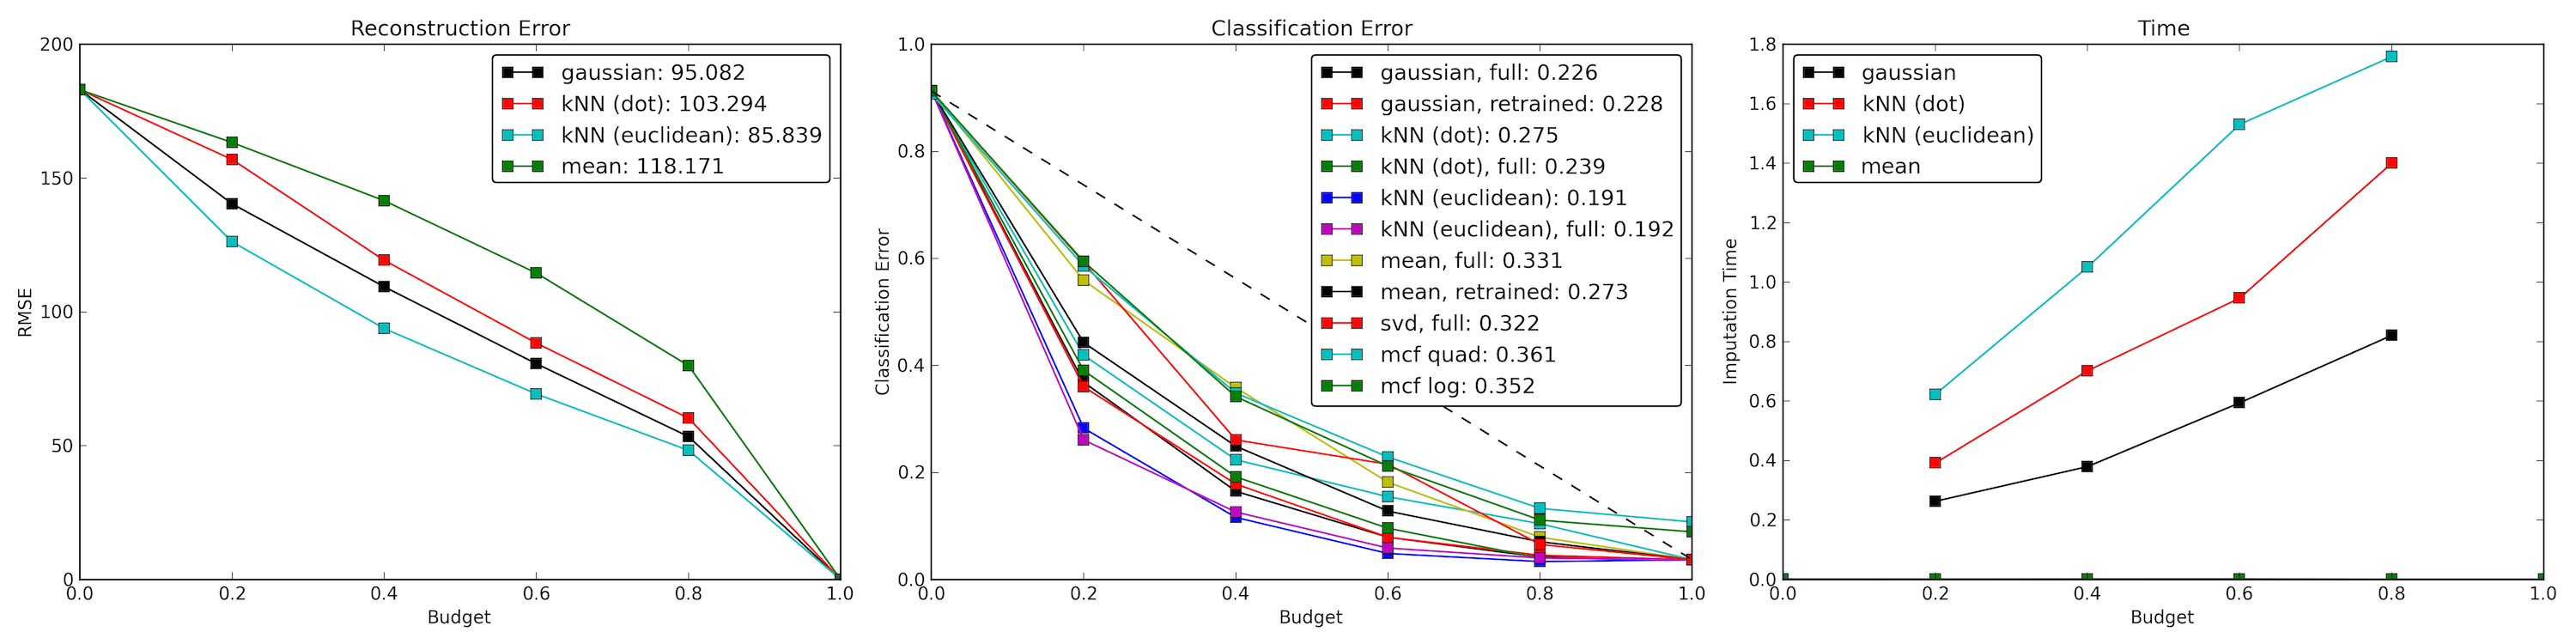
\includegraphics[width=1\textwidth]{../../figures/281b/digits_subplots.png}
  Random policy on the \textbf{Digits} dataset: $10$ classes with $200$ samples per class, feature dimension $64$ (pixels).
\end{center}

\begin{center}
  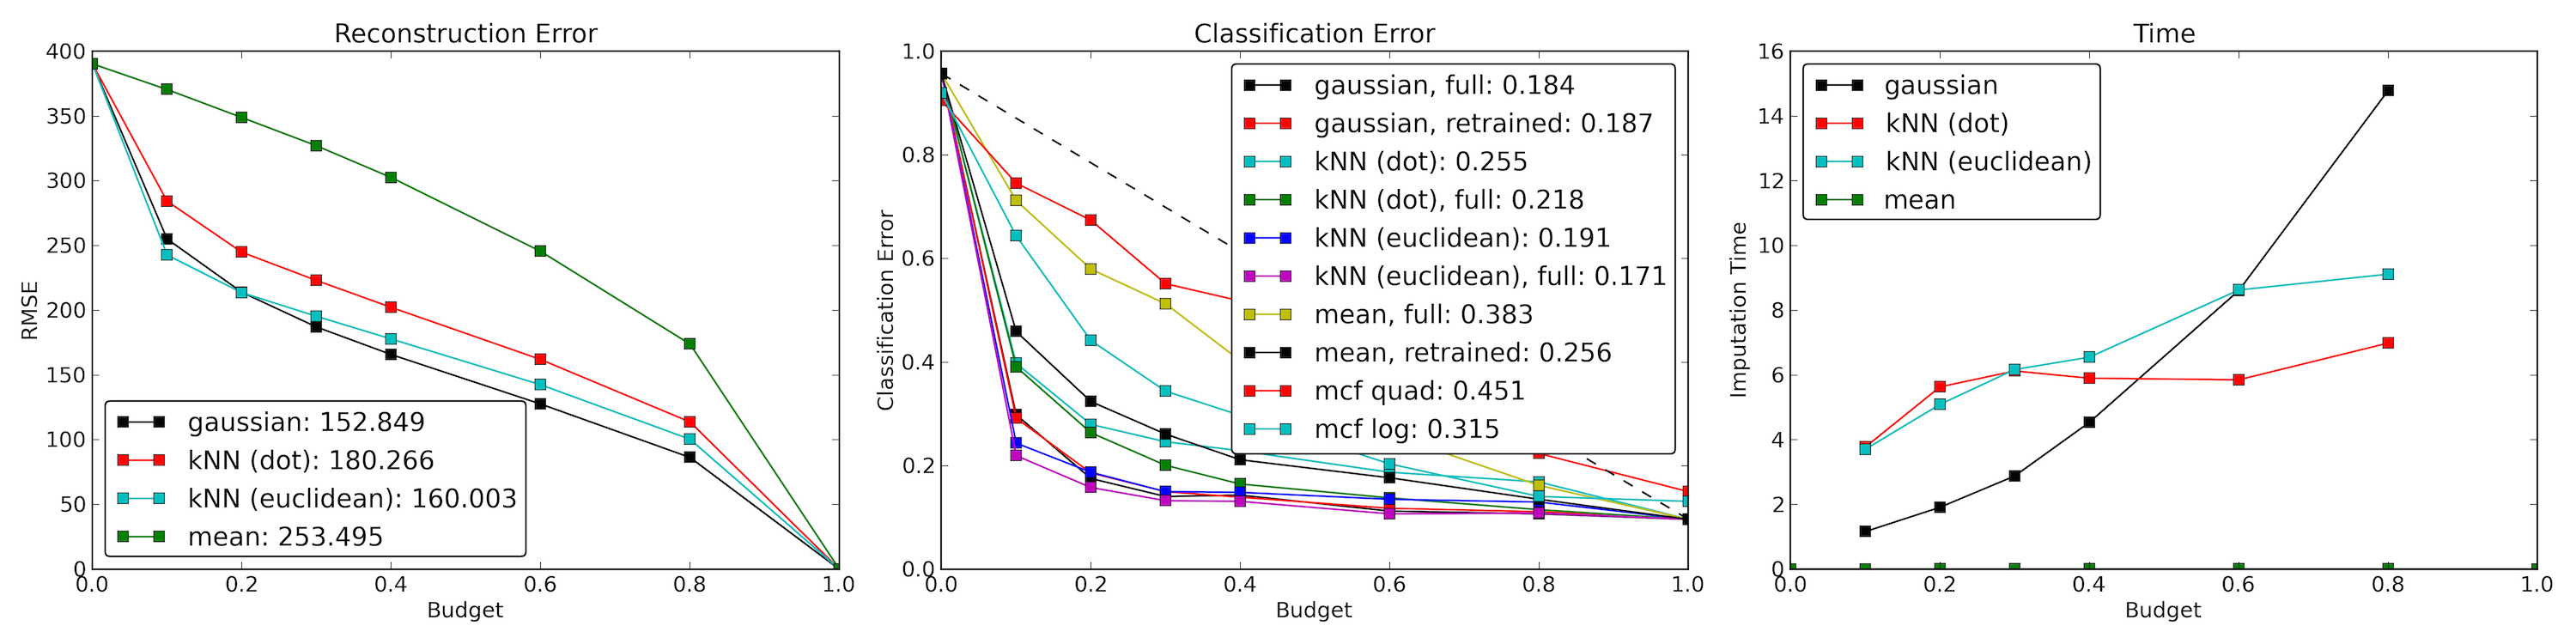
\includegraphics[width=1\textwidth]{../../figures/281b/scenes_subplots.png}
  Random policy on the \textbf{Scenes-15} dataset: $15$ classes, feature dimension is $165$ (SVM outputs of $11$ different feature kernels).
\end{center}

\begin{itemize}
\item The MCF loss classifier is outperformed by all approaches, including simple mean imputation with retraining.
\item Retraining the classifier with synthetically imputed data improves performance, but much more dramatically for simple approaches than for already well-performing imputations.
\item The most expensive method---$k$-NN---performs the best.
\end{itemize}
    }; \addcenteredtitle{results1}{Evaluation}

\end{tikzpicture}
\end{center}
\end{document}
